
\documentclass[twoside,a4paper]{article}
\usepackage{geometry}
\geometry{margin=1.5cm, vmargin={0pt,1cm}}
\setlength{\topmargin}{-1cm}
\setlength{\paperheight}{29.7cm}
\setlength{\textheight}{25.3cm}

% useful packages.
\usepackage{amsfonts}
\usepackage{amsmath}
\usepackage{amssymb}
\usepackage{amsthm}
\usepackage{enumerate}
\usepackage{graphicx}
\usepackage{multicol}
\usepackage{fancyhdr}
\usepackage{layout}
\usepackage{CJKutf8}

% some common command
\newcommand{\dif}{\mathrm{d}}
\newcommand{\avg}[1]{\left\langle #1 \right\rangle}
\newcommand{\difFrac}[2]{\frac{\dif #1}{\dif #2}}
\newcommand{\pdfFrac}[2]{\frac{\partial #1}{\partial #2}}
\newcommand{\OFL}{\mathrm{OFL}}
\newcommand{\UFL}{\mathrm{UFL}}
\newcommand{\fl}{\mathrm{fl}}
\newcommand{\op}{\odot}
\newcommand{\Eabs}{E_{\mathrm{abs}}}
\newcommand{\Erel}{E_{\mathrm{rel}}}

\begin{document}
\begin{CJK*}{UTF8}{gkai}

\pagestyle{fancy}
\fancyhead{}
\lhead{22035037 数学科学学院 计算数学专业}
\chead{数据结构作业 \#03}
\rhead{2020/10/20}


\section*{ 稳定快速排序算法的实现及平均时间效率测试}

\subsection*{a 问题} 

我们知道,标准的快速排序算法是不稳定的。其实有一些办法可以解决这个问题。比如,记录数据的原始下标,排完序后,对相同元素根据它们的原始下标,再排一次序。请你写程序实现这个算法。

\subsection*{b 文件说明}
由名为$main.cpp$的文件实现算法及测试,文件结构如下:

StableQuicksort

    |---class\_DATA

    |---function\_print
    
    |---function\_partition
    
    |---function\_quicksort
    
    |---function\_opti\_quicksort
    
    |---function\_stable\_opti\_quicksort
    
    |---function\_main
    
\noindent 其中,

|class\_DATA| 定义一个包含下标的数据类型;

|function\_print| 实现序列的输出,简化输出程序;

|partition| 实现快速排序中DATA类型序列按照val值进行的划分;

|quicksort| 递归地实现基于val值的快速排序;

|opti\_quicksort| 实现快速排序的同时避免在递归最底层依旧进行复杂的划分操作;

|stable\_opti\_quicksort| 实现稳定的快速排序——先对DATA类型序列按照val值进行原始的快速排序,再搜

\ \ 索排序后的序列中val值相同的数据,进行index指标的排序;

|main| 首先进行一组简单的排序测试以检验算法的正确性,其次通过对随机数序列的排序测试算法的复杂度,

\ \ 并生成两个data文件:平均运行时间data.avt及对应序列长度data.n。

\subsection*{c 测试步骤}
实现稳定算法的函数如下:

  int stable-opti-quicksort(DATA *arr, int n)
  
  {
    
    opti-quicksort(arr, n);
    
    DATA tmp;
    
    for(int i = 0; i < n-1; i++){
      
      if(arr[i].val == arr[i+1].val $ \& \& $ arr[i].index > arr[i+1].index){
        
        tmp = arr[i];
        
        arr[i] =arr[i+1];
        
        arr[i+1] = tmp;
        
      }
      
    }
    
    return 0;
    
}

\noindent a. 首先进行简单的测试

Before: A = [ 0:3.14159, 1:3.14159, 2:2.71828, 3:0, 4:1];
 
After: A = [ 3:0, 4:1, 2:2.71828, 0:3.14159, 1:3.14159];

排序结果正确。

\noindent b. 分析算法的平均代价:
  
根据static\_opti\_quicksort函数的构造,在opti\_quicksort函数的基础上增加了一个$O(n)$的$for$循环,因此算法的平均代价依然是$O(n \log n)$,可能对应的斜率和截距会比原始快速排序算法大一些,下面通过对随机数进行排序验证此结论;
  
  1. 测试规则:

  (1)依次生成n = 100,200,300,...,1000维[0.0,1.0]间的随机序列,每个n生成10个随机序列;
  
  (2)以上每个随机序列中的每一个随机数都重复十次,由此每个n得到10个维数为10*n的随机序列,同一n值得到

  \ \ \ \ \ \ \ 的运行时间进行平均作为平均代价的衡量标准(测试需要考虑出现相同数值时排序算法的稳定性,因此重复

  \ \ \ \ \ \ \ 值的出现在此次测试中是必要的);
  
  (3)对上述生成的随机序列分别利用opti\_quicksort和stable\_opti\_quicksort两种算法进行排序,最后可进行平均代

  \ \ \ \ \ \ \ 价的比较。
  
  2. 测试结束会生成数据文件“data.avt”和“data.n”,分别对应平均运行时间和相应的n值;
  
  3. 在 Matlab 中运行:
  
   hold on;
  
  plot(nlogn, T1,'black','LineWidth',1);
  
  plot(nlogn, T2,'r','LineWidth',1);
  
  xlabel('nlogn');
  
  ylabel('time');
  
  legend('stable-opti-quicksort','opti-quicksort');
  
  
\subsection*{d 数值结果}

\begin{figure}[htbp]
  \centering
  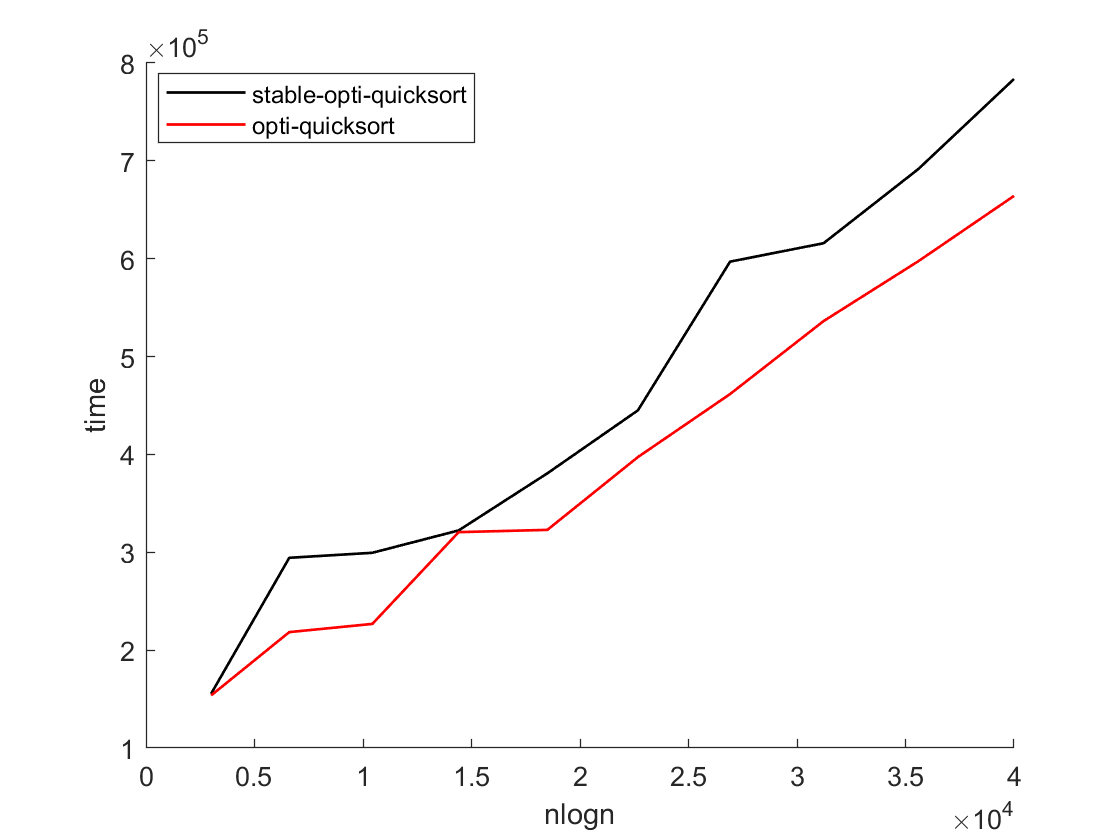
\includegraphics[width=0.5\textwidth]{plot.png}
  \caption{对比图}
  \label{fig:}
\end{figure}
\subsection*{e 结论}

实验结果验证了理论结果,这个稳定快速排序算法的平均代价是 $O(n \log n)$。



\end{CJK*}
\end{document}

%%% Local Variables: 
%%% mode: latex
%%% TeX-master: t
%%% End: 
